\documentclass[final,hyperref={pdfpagelabels=false}]{beamer}
\usepackage{grffile}
\mode<presentation>{\usetheme{UoL}}
\usepackage[english]{babel}
\usepackage[T1]{fontenc} 
\usepackage[utf8]{inputenc}
\usepackage{amsmath,amsthm, amssymb, latexsym}
\usepackage[scaled=0.98]{helvet}
\usepackage{layouts}
\usepackage{wrapfig}
\usepackage[caption=false,font=footnotesize]{subfig}


%\usepackage{times}\usefonttheme{professionalfonts}  % obsolete
%\usefonttheme[onlymath]{serif}
\boldmath
\usepackage[orientation=landscape,size=a0,scale=0.9]{beamerposter}
\usepackage{wrapfig}
\usepackage{comment}
% change list indention level
\setdefaultleftmargin{5em}{}{}{}{}{}

\usepackage[
backend=biber,
natbib=true,
style=numeric,
sorting=none]{biblatex}

\addbibresource{refs.bib}

%\usepackage{snapshot} % will write a .dep file with all dependencies, allows for easy bundling

\usepackage{array,booktabs,tabularx}
\newcolumntype{Z}{>{\centering\arraybackslash}X} % centered tabularx columns
\newcommand{\pphantom}{\textcolor{ta3aluminium}} % phantom introduces a vertical space in p formatted table columns??!!
\usepackage{parcolumns}

\listfiles

%%%%%%%%%%%%%%%%%%%%%%%%%%%%%%%%%%%%%%%%%%%%%%%%%%%%%%%%%%%%%%%%%%%%%%%%%%%%%%%%%%%%%%
\graphicspath{{../../Figures/}{./figures/}}

\title{\huge An Investigation into Physical and Communications Trust Frameworks \\
for Collaborative Teams of Autonomous Underwater Vehicles}
\author{Andrew Bolster, Prof. Alan Marshall, Prof. Jean-Guy Fontaine }
\institute[UoL]{Advanced Networks Research Group, University of Liverpool, UK}
\date[03/07/14]{July 3rd, 2014}

%%%%%%%%%%%%%%%%%%%%%%%%%%%%%%%%%%%%%%%%%%%%%%%%%%%%%%%%%%%%%%%%%%%%%%%%%%%%%%%%%%%%%%


\def\colwidth{0.2\linewidth}

\usecaptiontemplate{
\small
\structure{\insertcaptionname~\insertcaptionnumber:}
\insertcaption
} 
%%%%%%%%%%%%%%%%%%%%%%%%%%%%%%%%%%%%%%%%%%%%%%%%%%%%%%%%%%%%%%%%%%%%%%%%%%%%%%%%%%%%%%
\begin{document}
\begin{frame}[fragile]
	\begin{columns}[T]
		% ---------------------------------------------------------%
		% Set up a column 
		\begin{column}{\colwidth}
			\begin{beamercolorbox}[center,wd=\textwidth]{postercolumn}
				\begin{minipage}[T]{.98\textwidth}  % tweaks the width, makes a new \textwidth
					\parbox[t]{\textwidth}{ % must be some better way to set the the height, width and textwidth simultaneously
						% Since all columns are the same length, it is all nice and tidy.  You have to get the height empirically
						% ---------------------------------------------------------%
						% fill each column with content            
						%%%%%%%%%%%%
						\begin{block}{Project Background and Outputs}
							\begin{itemize}
								\item Attendance at UComms 2012 (Sestri Levante, Italy)
								\item Poster Presentations in 2012 (Kassam, Oxford) and 2013 (Heathrow, London and Bagneaux, Paris)
								\item Summer Research Placement with DSTL (Software Systems and Dependability for Autonomous Teams)(2013, Portsdown West, Portsmouth)
								\item Short Paper Presentation to the Association for the Advancement of Artificial Intelligence (AAAI) on ``A Multi Vector Trust Framework for Autonomous Systems'' (2014, Stanford, CA)\cite{Bolster2014}
								\item Technical Report for the UK/US/CAN/AUS/NZ Technical Cooperation Programme ((2014). Analysis of Trust Interfaces in Autonomous and Semi-Autonomous Collaborative MHPC Operations. The Technical Cooperation Program, Technical Report TR-C3I-06-2014) (June 13 - April 14)\cite{Bolster2014a}
								\item DSTL CDE Collaboration with NPL and Plextek Ltd. on ``Precision Timing and Navigation, Challenge 1: Resilient Time and Location Estimation for Networked Assets'' (CDE 33135) (Oct 13-May 14)
							\end{itemize}
						\end{block}
						
						%%%%%%%%%%%%
						\begin{block}{Introduction}
							\emph{Aim of project}: To combine physical and communications observations to assess and maintain trust within mobile, marine, ad-hoc networks
							
							\vspace{0.3\baselineskip}
							
							Small fleets of AUVs (\emph{Autonomous Underwater Vehicles}) will be expected to operate in isolated environments.
							\vspace{0.3\baselineskip}
							
							This requires an auditable sense of trust within the remote intra-fleet communications networks, incorporating
							\begin{itemize}
								\item Communications Activity
								\item Mission Suitability/Capability
								\item Behavioural Monitoring
							\end{itemize}
							
							\vspace{0.3\baselineskip}
							
							The use of centrally coordinated trust models presents a single point of failure.
							
							\vspace{0.3\baselineskip}
							
							Secure communication in marine environments is expensive and time consuming; adopting a decentralised form of trust assurance will reduce these costs by localising the per-node security environment.
							
							\begin{figure}[h]
								\centering
								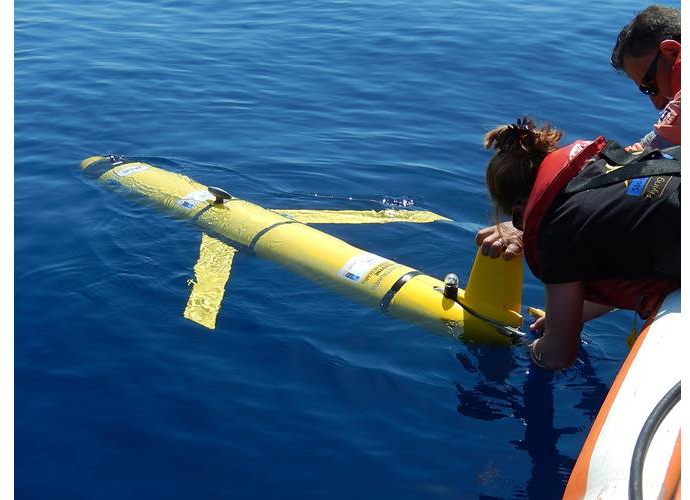
\includegraphics[width=0.6\linewidth]{remus100cmre}
								\vspace{1ex}
								\caption{REMUS 100 AUV, as deployed at CMRE, a potential target platform for this work}
							\end{figure}
						\end{block}
						%%%%%%%%%%%%
						\begin{block}{Trust}
							Trust is:
							\begin{itemize}
								\item \emph{The expectation of an actor performing a certain task or range of tasks within a certain confidence or probability}
								\item a belief on the reliability of an entity
								\item based on both direct and indirect historical experience
							\end{itemize}
							\vspace{0.3\baselineskip}
							
							Individual trust opinions are shared within the network concerning a range of activities:
							\begin{itemize}
								\item Transmission Relaying (Local and/or Backhaul)
								\item Position Relaying
								\item Reporting Accuracy
							\end{itemize}
							\vspace{0.3\baselineskip}
							
							These Trust opinions also apply to extra-fleet entities, such as surface platforms, submarine comms links, and coastal stations, allowing the fleet to collaboratively form an opinion of these actors.
							
						\end{block}
					}
				\end{minipage}
			\end{beamercolorbox}
		\end{column}
		% ---------------------------------------------------------%
		% end the column
		
		% ---------------------------------------------------------%
		% Set up a column 
		\begin{column}{\colwidth}
			\begin{beamercolorbox}[center,wd=\textwidth]{postercolumn}
				\begin{minipage}[T]{.98\textwidth} % tweaks the width, makes a new \textwidth
					\parbox[t]{\textwidth}{ % must be some better way to set the the height, width and textwidth simultaneously
						% Since all columns are the same length, it is all nice and tidy.  You have to get the height empirically
						% ---------------------------------------------------------%
						% fill each column with content
						%%%%%%%%%%%%
						\begin{block}{Trust Management Frameworks (TMFs)}
							
							TMFs are protocols designed to provide information regarding the estimated future states and operations of nodes within networks
							\vspace{0.3\baselineskip}
							
							``[\ldots]collecting the information necessary to establish a trust relationship and dynamically monitoring and adjusting the existing trust relationship'' - \cite{Li2007}
							\vspace{0.3\baselineskip}
							
							\begin{columns}[T]
								\begin{column}{0.45\textwidth}
									Enables nodes to form collaborative \emph{opinions} on their cohort nodes based on
									\begin{itemize}
										\item Direct Observation of Communications Behaviour (eg Successfully Forwarded Packets)
										\item Common-Neighbour Recommendation
										\item Indirect Reputation
									\end{itemize}
								\end{column}
								\begin{column}{0.45\textwidth}
									\begin{figure}[H]
										\centering
										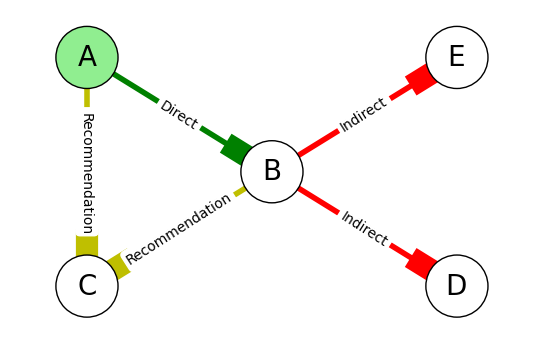
\includegraphics[width=\linewidth]{node_relationships}
										\vspace{1ex}
										\caption{Direct, Recommendation, and Indirect trust relationships}
									\end{figure}
								\end{column}
							\end{columns}
							
							\vspace{0.3\baselineskip}
							
							Multiple transitive relationships can be maintained over time, providing trust resilience with dynamic network topologies 
							
						\end{block}
						%%%%%%%%%%%%
						\begin{block}{The Need for Multi-Domain Trust in Autonomous Systems}
							Communications not the only target for an attacker (or failure);
							\begin{itemize}
								\item Following to restricted area
								\item Masquerading
								\item Hardware Degradation
								\item Resource attack via propulsive power
							\end{itemize}
							Physical observation presents opportunity to further reduce the available threat surface while also discriminating between 'True' attacks and mechanical failure.
							
							\vspace{0.3\baselineskip}
							
							Potential attacks exist within a multi-domain threat surface, and as further metrics and domains of trust are included in a TMF, attackers are increasingly restricted in their behaviour until the only way to avoid detection is to behave correctly.
							\begin{figure}[h]
								\centering
								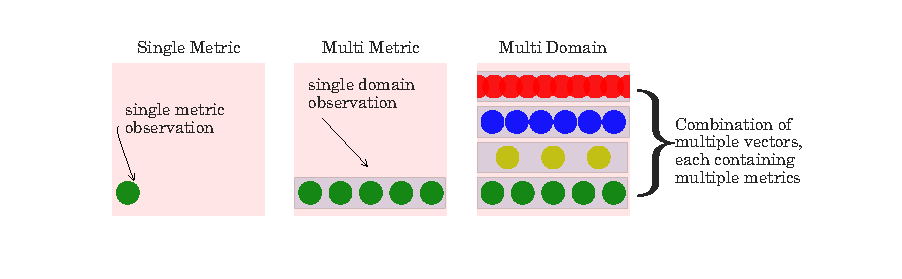
\includegraphics[width=0.9\linewidth]{threat_surface_sum}
								\caption{Threat Surface for Trust Management Frameworks}
							\end{figure}
						\end{block}
						
						
						%%%%%%%%%%%%
						\iffalse
						\begin{block}{Base Collision avoidance behaviour (Boid-like flocking)}
							\begin{columns}[T]
								\begin{column}{.70 \textwidth}
									Simple Boidean flocking is used to provide a safe 
									\begin{itemize}
										\item Cohesion
										\begin{equation}
											F_{j,C}= F_A\left(p_j, \frac{1}{N}\sum\limits_{\forall i \ne j}^N{p_i}, d_{max}\right)
										\end{equation}
										\item Repulsion
										\begin{equation}
											F_{j,H}= \sum\limits_{\forall i \ne j}^N F_R\left(p_j, p_i, d_{max}) \big| d_{max}>\|p_i-p_j\|\right)
										\end{equation}
										\item Alignment
										\begin{equation}
											F_{j,CA}= \frac{1}{N}\cdot\left(\sum\limits_{\forall i \ne j}^N \hat{v_i}\right) 
										\end{equation}
									\end{itemize}
								\end{column}
								\begin{column}{.25\textwidth}
									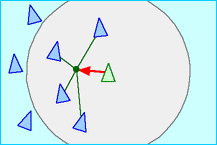
\includegraphics[width=0.9\textwidth]{figures/flocking_cohesion.gif}
									\vspace{0.3\baselineskip}
									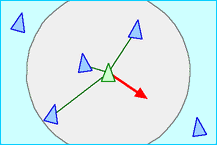
\includegraphics[width=0.9\textwidth]{figures/flocking_separation.gif}
									\vspace{0.3\baselineskip}
									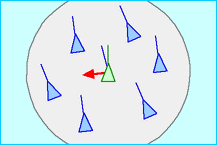
\includegraphics[width=0.9\textwidth]{figures/flocking_alignment.gif}
								\end{column}
							\end{columns}
							\vspace{0.3\baselineskip}
							Where $F_A$ is a scaled vector attraction function, and $F_R$ is an equivalent repulsion function
						\end{block}

            \fi
						%%%%%%%%%%%%

            %%%%%%%%%%%%
						\begin{block}{Multi-Metric Trust Assessment}
              Most TMFs can be generalised as single-metric estimators based on a binary input stats (Packet Loss/Delivery Rates), which provides malicious actors advantage if their activity does not affect that metric. MTFM\cite{Guo11} analyses more than PLR to make it's assessment, including Received and Transmitted signal strength, delay, and throughput as well as taking account of dynamic network topology to inform assessment.

                \begin{align}
                  \label{eq:grc}
                  [\theta_{k,j}^t,\phi_{k,j}^t]  &= \frac{\min_k|a_{k,j}^t - r_j^t| + \rho \max_k|a_{k,j}^t-r_j^t|}{|a_{k,j}^t-r_j^t| + \rho \max_k|a_{k,j}^t-r_j^t|},  r \in [g,b]\\
                  \label{eq:metric_weighting}
                  [\theta_k^t, \phi_k^t] &= \left[\sum_{j=0}^M h_j \theta_{k,j}^t,\sum_{j=0}^M h_j \phi_{k,j}^t \right]\\
                  \label{eq:trust_value}
                  T_k^t &= ({1+{(\phi_k^t)^2}/{(\theta_k^t)^2}})^{-1}
                \end{align}
                where $a_{k,j}^t$ is the value of an observed metric $x_j$ for a given node $k$ at time $t$, $\rho$ is a distinguishing coefficient set to $0.5$, $g$ and $b$ are respectively the ``good'' and ``bad'' reference metric sequences from $a$, i.e. $g_j=\max_k({a_{k,j}^t})$,  $b_j=\min_k({a_{k,j}^t})$ 

                These metric coefficients are then accumulated \eqref{eq:metric_weighting} and combined to present a singular trust value for analysis \eqref{eq:trust_value}.

                The weights used in \eqref{eq:metric_weighting} can be used to interrogate the trust value space, putting more emphasis on one or more metrics to identify and better characterise a misbehaviour.

						\end{block}

						
						
					}
				\end{minipage}
			\end{beamercolorbox}
		\end{column}
		% ---------------------------------------------------------%
		% end the column
		
		% ---------------------------------------------------------%
		% Set up a column 
		\begin{column}{\colwidth}
			\begin{beamercolorbox}[center,wd=\textwidth]{postercolumn}
				\begin{minipage}[T]{.98\textwidth} % tweaks the width, makes a new \textwidth
					\parbox[t]{\textwidth}{ % must be some better way to set the the height, width and textwidth simultaneously
						%%%%%%%%%%%%
						\begin{block}{Operational Mission Profiles}
							Generic behaviours currently under investigation include:
							\begin{itemize}
								\item \emph{Waypointing} - Attraction to a point or a chain of points, providing pre-described patrol networks
								\item \emph{Surveying} - Fleets can be tasked to provide one-shot, or persistent coverage of an area of the environment utilising a dynamic lawnmower pattern.
								\item \emph{Dynamic Constraint} - Repulsion from a series of points, analogous to sea-borders or shipping lanes.
							\end{itemize}
							
							Potentially Exploitable Behaviours not yet developed include:
							\begin{itemize}
								\item \emph{Capacity Based Homing} - Where a node leaves and later returns to the fleet, for instance for refuelling or resupply.
								\item \emph{Dynamic Communications Maintenance} - The fleet can adjust to changing communications environments.
							\end{itemize}
						\end{block}
						%%%%%%%%%%%%
						\iffalse
						\begin{block}{Malicious Behaviours}
							A series of 'Malicious' behaviours have been designed, where one or more nodes were actively attempting to compromise the fleet in some way.
							\begin{itemize}
								\item \emph{Shadow} - Following the fleet without restricted mission data
								\item \emph{Spy} - A node that intermittently rises in the fleet, potentially surfacing to relay mission information to a third party
								\item \emph{Sloth} - Selfish conservation of energy by taking minimal paths
								\item \emph{Stalker} - Tailing a specific node, attempting to use this consistent history to poision the trust network
								\item \emph{Scoundrel} - Falsely reporting its estimated position with the intention to corrupt a collaborative positioning system or induce a collision
							\end{itemize}
							
							Additionally, there are non-malicious behaviours, the classification of which is equally important in separating friend from foe.
							\begin{itemize}
								\item \emph{Slow Coach} - Where a node's power train is damaged, causing reduced maneuverability and performance
								\item \emph{Spin Doctor} - Damage to control surfaces or to Inertial Navigation System
							\end{itemize}
							
						\end{block}
						
						%%%%%%%%%%%%
						\begin{block}{Simulation Framework}
							Bespoke Simulation framework consisting of three modules:
							\begin{itemize}
								\item \texttt{Aietes} : the original base behavioural simulator, performing agent-based modelling of the motions of AUV's within an 
								environment
								\item \texttt{Bounos} : a collection of data processing and collation functions.
								\item \texttt{Ephyra} : a GUI visualisation (and later, control) system for both Aietes and Bounos (See Fig~\ref{fig:Ephyra})
							\end{itemize}
							
							\vspace{0.3\baselineskip}
							
							It is highly flexible, allowing for:
							\begin{itemize}
								\item Arbitrary node configurations (both in terms of physical and communications capabilities)
								\item Generically Based on the REMUS 100 configuration and physical model, but extendible to other dynamics
								\item Support for runtime and \emph{a-posteriori} statistical analysis with numpy/scipy/pandas
								\item Componentised Behaviour network, with a Boid-like collaborative control path base behaviour (flocking)
								\item Integration to the SUNSET emulation platform, allowing for rapid integration to real equipment
							\end{itemize}
							\vspace{\lineskip}
							\begin{figure}
								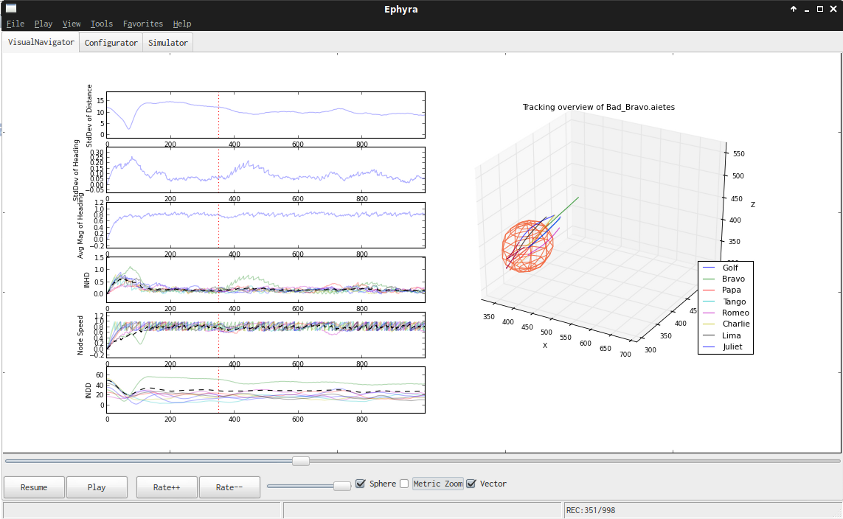
\includegraphics[width=0.9\textwidth]{figures/ephyra_vis}
								\caption{The Ephyra visualiser built with WxPython allows for rapid modelling and analysis of multi-dimensional vector data, in this case showing a interactive real-time 3D model of the fleet positions and trails, as well as overlay information on individual and fleet behaviours, and on the left, fleet- and node- level metrics plotted over time.}
								\label{fig:Ephyra}
							\end{figure}
						\end{block}     
						\fi
						%%%%%%%%%%%%
						
						%%%%%%%%%%%%
						\begin{block}{Behavioural Analysis}
							Three fleets are simluated performing a simple 8 hour duration patrol mission. The first includes a malicious node attempting to infiltrate the fleet (Shadow). The second has an impared or faulty but otherwise "good" node (SlowCoach). The third is a baseline fleet with all "Good" nodes
							
							\vspace{0.3\baselineskip}
							
							Physical Metrics under assessment:
							\begin{itemize}
								\item \emph{INHD}: Inter Node Heading Deviation, or the per-node variation from the fleet-average direction
								\item \emph{Node Speed}: The Magnitude of Velocity of each node compared to the fleet-average
								\item \emph{INDD}: Inter Node Distance Deviation, or the variation between the inter-node distances between each node
							\end{itemize}
							
							\vspace{0.3\baselineskip}
							
							In this initial model, there are no 'positive' trust expression; all nodes are 'distrusted' to some degree dependant on consistent or periodic deviation from fleet norms.
							
							\begin{figure}
								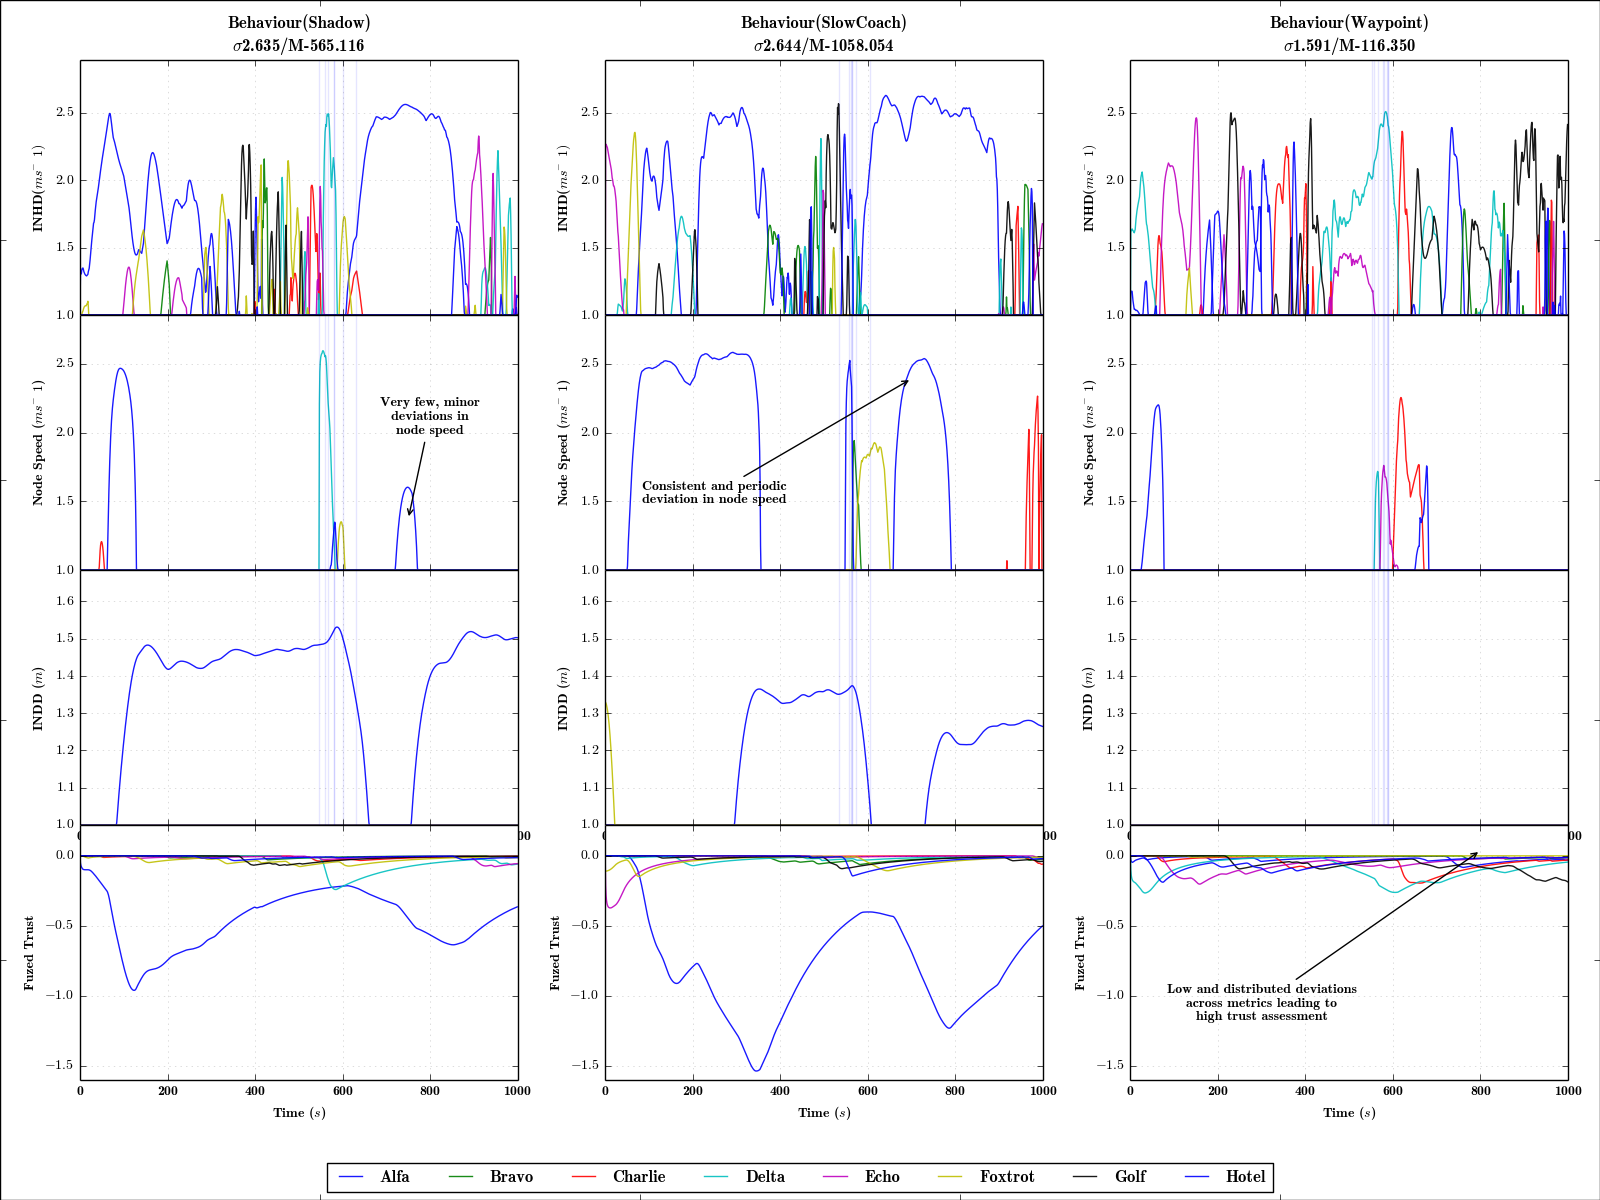
\includegraphics[width=0.95\textwidth]{figures/Bad_Alfa_Fusion}
								\caption{Per-Node deviations for each metric, with an additional row showing an EWMA based cross-metric trust assessment. Annotations highlight difference in 'Node Speed' triggers between the malicious and impaired behaviours }
								\label{fig:Bad_Alfa_Fusion}
							\end{figure}
							
              From Fig. ~\ref{fig:Bad_Alfa_Fusion}, \emph{INDD} is a clear candidate for a suspicion 'trigger', but looking at \emph{INHD} values after several minutes of mission time; an anomaly is clearly being detected. 
							
							\vspace{0.3\baselineskip}
							
							In addition, \emph{Alfa} node (Blue) is clearly an outlier in terms of \emph{INHD} and \emph{Node Speed} in the earliest sections of the graph. This implies that a fusion of metrics would be more effective than a simple detection envelope on a single metric.
							
							
							Considering the baseline Waypointing results in Figure ~\ref{fig:Bad_Alfa_Fusion}, it's clear that these metrics are not infallible, as is demonstrated by the number of relatively short-lived false positives, demonstrating the need to use multiple metrics for reliable trust assessment.
							
							\vspace{0.3\baselineskip}
							
							Figure ~\ref{fig:Bad_Alfa_Fusion} demonstrates a windowed, weighted trust fusion, where deviations in individual metrics are combined to generate a Trust Value. 
						\end{block}
						%%%%%%%%%%%%
					}
					% ---------------------------------------------------------%
					% end the column
				\end{minipage}
			\end{beamercolorbox}
		\end{column}
		% ---------------------------------------------------------%
		
		% ---------------------------------------------------------%
		% Set up a column 
		\begin{column}{\colwidth}
			\begin{beamercolorbox}[center,wd=\textwidth]{postercolumn}
				\begin{minipage}[T]{.98\textwidth} % tweaks the width, makes a new \textwidth
					\parbox[t]{\textwidth}{ % must be some better way to set the the height, width and textwidth simultaneously
						% Since all columns are the same length, it is all nice and tidy.  You have to get the height empirically
						% ---------------------------------------------------------%
						% fill each column with content
						%%%%%%%%%%%%
						\begin{block}{Single and Multi-Metric TMF operation in Marine Comms}
                Acoustic Network based on AUVNetSim \cite{Miquel2008} and validated against \cite{Stefanov2011}.

                \vspace{0.3\baselineskip}
							
                Aim to investigate use of Multi-Parameter Trust Framework for MANETS (MTFM), against current communications TMFs (Hermes/ Objective Trust Management Framework (OTMF)), which exclusively use Packet Loss Rate (PLR) as their assessment metric.  

                \vspace{0.3\baselineskip}
							
                Two Communications Misehaviours were generated:
                \begin{itemize}
                  \item \textbf{Malicious Power Control}(MPC) where a malicious node ($n_1$) inflates it's power to all nodes except a target node ($n_0$) such that that node appears to be behaving selfishly.
                  \item \textbf{Selfish Target Selection}(STS) where $n_1$ preferentially communicates with nodes that are physically near-by, reducing its own power consumption.
                \end{itemize}

                \begin{figure}[t]
                  \subfloat[Fair Scenario]{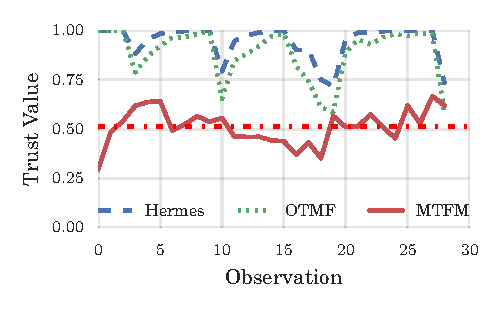
\includegraphics[width=.33\linewidth]{trust_beta_otmf_fair} \label{fig:all_mobile_fair_beta}}
                  \subfloat[MPC Scenario]{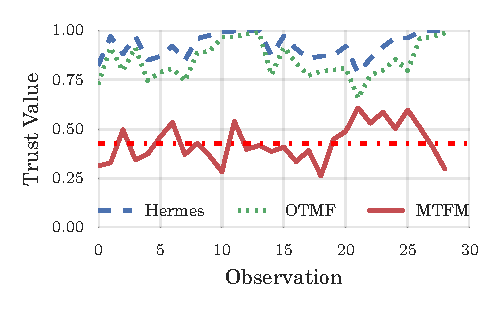
\includegraphics[width=.33\linewidth]{trust_beta_otmf_malicious} \label{fig:all_mobile_badmouthing_beta}}
                  \subfloat[STS Scenario]{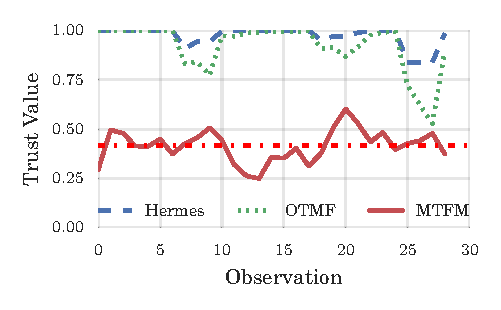
\includegraphics[width=.33\linewidth]{trust_beta_otmf_selfish} \label{fig:all_mobile_selfish_beta}}
                  \caption{$T_{1,0}$ for Hermes, OTMF and MTFM assessment values for fair and malicious behaviours in the fully mobile scenario (mean of MTFM also shown)}
                  \label{fig:otmf_beta_comparison}
                \end{figure}

                From ~\ref{fig:otmf_beta_comparison}, in the challenging underwater environment, no assessment tool is able to appreciably differentiate between behaviours (while MTFM does display a 10\% discriminating behaviour in the a-postori average assessment, shown as a red dashed line)

                                Metric suitability for trust assessment using a distributied weighting analysis using Random Forest Regression Techniques.



						\end{block}
						%%%%%%%%%%%%

						%%%%%%%%%%%%
						\begin{block}{Future Applications}
							\begin{itemize}
								\item Due to the high communications, motion, and computation costs, and lack of external location reporting (\emph{e.g. GPS}), 
								behavioural analysis in the marine environment is particularly difficult, but if successful, can be reliably applied in a wide 
								variety of fields including but not limited to
								\begin{itemize}
									\item Self-Driving Cars
									\item Environmental Survey drones (terrestrial, marine, and aerial)
									\item Satellite Communications Arrays
									\item Internet Certificate Authority verification
									\item Verifiable Distributed Computing
								\end{itemize}
							\end{itemize}              
						\end{block}
						%%%%%%%%%%%%
						
					}
					% ---------------------------------------------------------%
					% end the column
				\end{minipage}
			\end{beamercolorbox}
		\end{column}
		% ---------------------------------------------------------%
		% end the column   % end the column
		% ---------------------------------------------------------%
		% Set up a column 
		\begin{column}{\colwidth}
			\begin{beamercolorbox}[center,wd=\textwidth]{postercolumn}
				\begin{minipage}[T]{.98\textwidth} % tweaks the width, makes a new \textwidth
					\parbox[t]{\textwidth}{ % must be some better way to set the the height, width and textwidth simultaneously
						% Since all columns are the same length, it is all nice and tidy.  You have to get the height empirically
						% ---------------------------------------------------------%
						% fill each column with content
						%%%%%%%%%%%%
						
						\begin{block}{Conclusions}
							This research area presents a range of challenges and opportunities within both civil and defence operations; an auditable trust framework for automated marine craft would be a significant enabling factor to the roll-out of more low-maintenance or even ``Fire and Forget'' deployments for persistent patrol/monitoring tasks. 
							
							\vspace{0.3\baselineskip}
							
							Open Hypotheses in this field that this project intends to answer are:
							\begin{itemize}
								\item How can optimality in trust assessment based on behaviour be defined win a distributed, dynamic network topology?
								\item Is there a quantifiable benefit to cross-domain comparison beyond single-vector trust? (i.e. 1-D vector vs cross domain comparison)
								\item Is there an optimal \emph{generic} cross domain fusion methodology?
							\end{itemize}
						\end{block}
						%%%%%%%%%%%%
						\begin{block}{Development Plan}
							\begin{itemize}
								\item Behaviour Detection (Q3 14) - Formal Analysis of Behavioural Trust Systems
								\begin{itemize}
									\item ASON 2014 : Seventh Int. WS on Autonomous Self-Organizing Networks (Aug 14)
									\item AHUC 2014 : The Fourth Int. WS on Ad Hoc and Ubiquitous Computing (Aug 14)
									\item ICCAR 2015 : WASET Int. Conf. on Control, Automation and Robotics (Dec 14)
								\end{itemize}
								\item MANET/Marine comparison (Q4 14) - Formal Comparison between Terrestrial MANET / Marine contexts
								\item Multi-Domain Trust Assessment (Q4 14) - Combination of Communicative and Physical Behaviour Trusts
								\begin{itemize}
									\item IEEE Trans. on Communications / Dependable and Secure Computing / Intelligent Systems
								\end{itemize}
								\item Reactionary/Perturbative Trust (Q1 15) - Exploration of reactionary behaviours for teams to 'shake down' suspects
								\begin{itemize}
									\item SASO15:Self-Adaptive and Self-Organizing Systems, 
									\item SEAMS15: Software Engineering for Adaptive and Self-Managing Systems
								\end{itemize}
							\end{itemize}
							
						\end{block}
						
						
						%%%%%%%%%%%%
						
						
						\begin{block}{Bibliography}
							
							\printbibliography[title=References]% [nottype=video]}
						\end{block}
					}
					% ---------------------------------------------------------%
					% end the column
				\end{minipage}
			\end{beamercolorbox}
		\end{column}
		% ---------------------------------------------------------%
		% end the column   % end the column
		
	\end{columns}
\end{frame}
\end{document}


%%%%%%%%%%%%%%%%%%%%%%%%%%%%%%%%%%%%%%%%%%%%%%%%%%%%%%%%%%%%%%%%%%%%%%%%%%%%%%%%%%%%%%%%%%%%%%%%%%%%
%%% Local Variables: 
%%% mode: latex
%%% TeX-PDF-mode: t
%%% End:
